\documentclass{article}

\usepackage[most]{tcolorbox}
\usepackage{physics}
\usepackage{graphicx}
\usepackage{float}
\usepackage{amsmath}
\usepackage{amssymb}


\usepackage[utf8]{inputenc}
\usepackage[a4paper, margin=1in]{geometry} % Controla los márgenes
\usepackage{titling}

\title{Clase 14}
\author{Manuel Garcia.}
\date{\today}

\renewcommand{\maketitlehooka}{%
  \centering
  \vspace*{0.05cm} % Espacio vertical antes del título
}

\renewcommand{\maketitlehookd}{%
  \vspace*{2cm} % Espacio vertical después de la fecha
}

\newcommand{\caja}[3]{%
  \begin{tcolorbox}[colback=#1!5!white,colframe=#1!25!black,title=#2]
    #3
  \end{tcolorbox}%
}

\begin{document}
\maketitle

\caja{black}{Revision taller }{
  \centering
  12 de octubre.
}
\section{Particula libre con potencial}
Tenemos una particula de masa $ m  $ que se encuentra atrapada en un segmento de recta $ L  $, la particula se encuentra en un pozo de potencial.
\begin{figure}[H]
  \begin{center}
    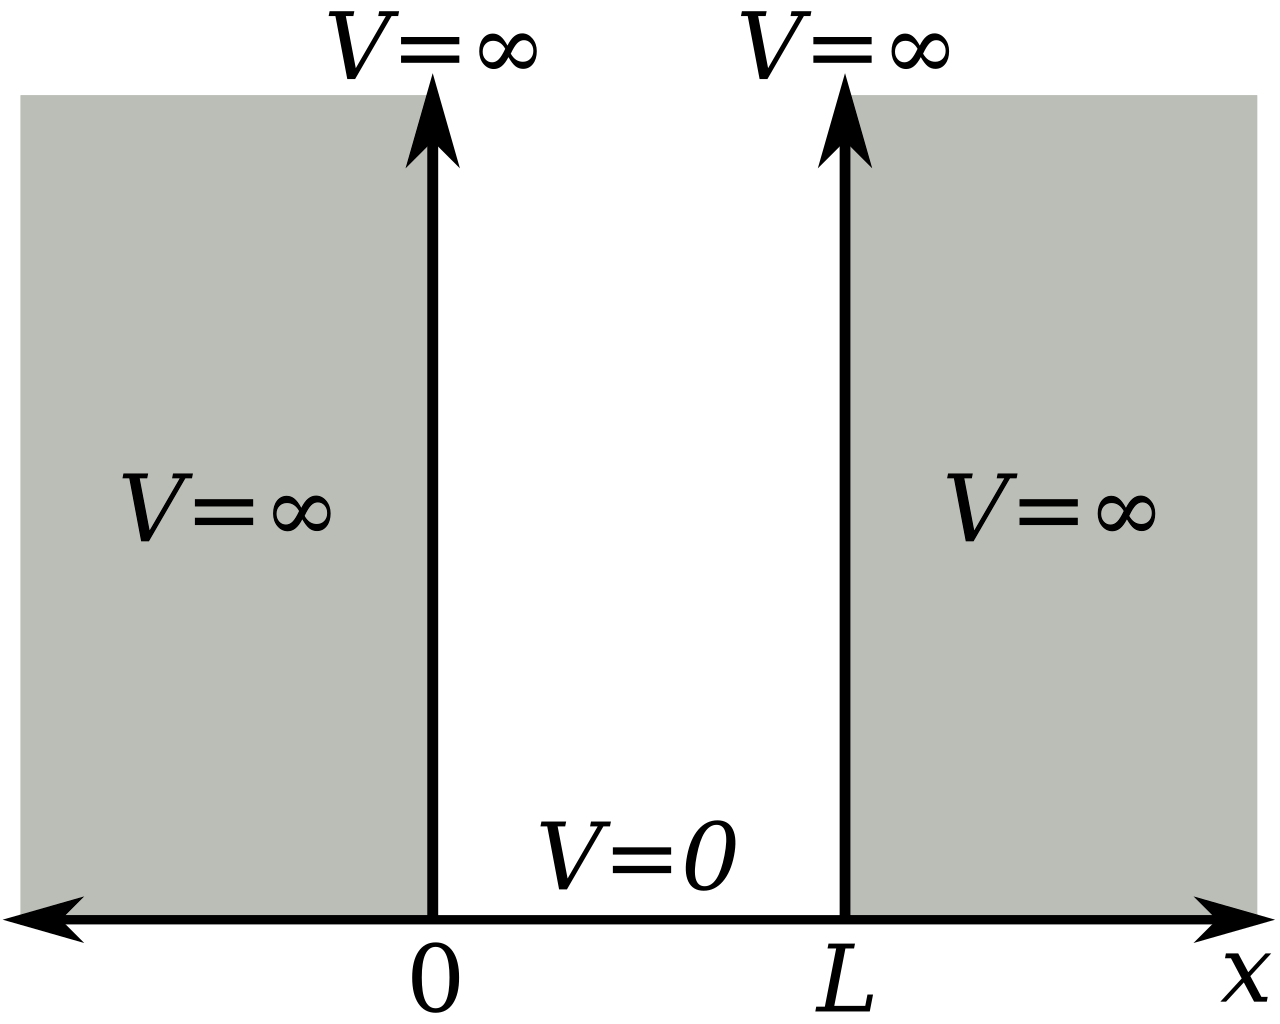
\includegraphics[width=0.25\textwidth]{pozo_potencial.png}
  \end{center}
\end{figure}
Esto lo podemos describir aplicando condiciones de frontera: 
\begin{gather*}
  \psi(L) = 0 \qquad \qquad \psi(0) = 0  
\end{gather*}
Tenemos $ H \ket{\psi} = E \ket{\psi}$ con $ H = \displaystyle\frac{p ^2}{2m } + V  $. 

Las condiciones de frontera que dimos anteriormente nos reemplaza el potencial por lo que podemos utilizar la ecuacion de la particula libre.
\begin{gather*}
  - \displaystyle\frac{\hbar ^2}{2m }\frac{d ^2  }{d x^2 }\psi(x) = E\psi(x) \quad \text{(ec. particula libre)} 
\end{gather*}
Por ejemplo en el oscilador armonico aplicamos que x tiende a infinito por lo que despreciamos el termino $ E\psi(x) $.

Para la ecuacion de la particula libre podemos encontrar la solucion: 
\begin{gather*}
  \psi(x) = A \sin{(\alpha x + \delta)}
\end{gather*}
Al aplicar esta solucion con las condiciones de frontera:
\begin{gather*}
  \displaystyle\frac{\hbar  ^2}{2m }\alpha ^2 = E \quad \rightarrow \quad \alpha = \pm \displaystyle\frac{\sqrt{2m E } }{\hbar } 
\end{gather*}
y $ \delta = 0  $.

Aplicando la primera condicion: 
\begin{gather*}
  \sin{\alpha L } = 0 \quad \rightarrow \quad \alpha L = m \pi \quad \rightarrow \quad \alpha L = m \pi 
\end{gather*}
Utilizando esto podemos dar el valor de la energia: 
\begin{gather*}
  E_n = \displaystyle\frac{1}{ 2m } \displaystyle\frac{(n \pi \hbar  ) ^2}{L ^2} 
\end{gather*}
Si tenemos $ m=0  $ tendriamos una funcion de onda nula por lo cual no representa ningún estado fisico.

Si hacemos $ n = n'+1 $ con $ n' = 0,1,2,...  $ podemos escribir la ecuacion para la energia como: 
\caja{red}{}{
  \begin{gather*}
    E_n = \displaystyle\frac{1}{2m }\displaystyle\frac{((n'+1) \pi \hbar  ) ^2}{L^2 } 
  \end{gather*}
  En la mayoria de los textos se toma la ecuacion para la energia de esta forma. 
}
Por lo tanto la funcion de onda para la particula libre con estas condiciones de frontera es: 
\caja{red}{}{
  \begin{gather*}
    \bra{x }\ket{n } =  \psi_n (x) = A \sin{\alpha x } 
  \end{gather*}
}
Calcular $ \psi(p)  $ no tiene sentido ya que como es la transformada de fourier tendiramos que integrar de $ -\infty $ a $ \infty $ con respecto a $ x $ pero nuestro problema solo está definido entre 0 y $ L  $ por lo que calcular $ \psi(p) $ no tiene sentido fisico. 
\caja{blue}{Ejercicio }{
  Encontrar que $ \psi_n (x) = A \sin{\displaystyle\frac{n \pi x }{L}} $.

  \textbf{Sol: }
  \begin{gather*}
    \alpha = \displaystyle\frac{\sqrt{2m E } }{\hbar } = \displaystyle\frac{\sqrt{2m \displaystyle\frac{1}{2m }\displaystyle\frac{(n \pi \hbar  ) ^2}{L^2 }} 
    }{\hbar } = \displaystyle\frac{n\pi}{L}
  \end{gather*}
}

$ A  $ es la constante de normalizacion
\begin{gather*}
  \bra{n' }\ket{n } = \delta _{n',n } \\
  \displaystyle\int_{0 }^{L } \bra{n }\ket{x }\bra{x }\ket{n }dx = \delta _{n',n } 
\end{gather*}

Este problema lo podemos generalizar a un caso tridimensional donde la particula se encuentra encerrada en un cubo de lado $ L  $.

\end{document}
